% Cho một đồ thị vô hướng $G = (V, E)$ và một tập các giá trị tần số nguyên dương $F = \{\dots\}$. Trong đó:
% \begin{itemize}
%     \item $V = \{1, 2, \dots, n\}$ là tập các đỉnh.
%     \item Mỗi đỉnh $i \in V$ có miền giá trị có thể nhận là $F_i \subseteq F$.
%     \item $E$ là tập các cạnh, mỗi cạnh $(u, v) \in E$ được gán một trọng số nguyên dương $d_{u,v}$.
% \end{itemize}

% Một nghiệm của bài toán là cách gán tần số $f(u) \in F_u$ cho mỗi đỉnh $u \in V$ sao cho với mỗi cạnh $(u, v, d_{u,v}) \in E$, ta có điều kiện: $|f(u) - f(v)| > d_{u,v}$ hoặc $|f(u) - f(v)| = d_{u,v}$ . Mục tiêu là tìm giá trị nhỏ nhất của số các tần số khác nhau được sử dụng.
% Dựa trên công trình nền tảng của Aardal và cộng sự \cite{Aardal2007}, bài toán gán tần số tối thiểu hóa (MO-FAP) có thể được mô hình hóa trực tiếp thông qua Quy hoạch tuyến tính nguyên (Integer Linear Programming - ILP). Gọi $G=(V, E)$ là đồ thị mạng lưới với $V$ là tập các đỉnh (trạm phát sóng) và $E$ là tập các cạnh thể hiện khả năng gây nhiễu tín hiệu. Gọi $F$ là tập các tần số vô tuyến khả dụng. Với hai tập biến quyết định nhị phân $x_{vf}$ (nhận giá trị 1 nếu gán tần số $f$ cho đỉnh $v$, và 0 nếu ngược lại) và $y_f$ (nhận giá trị 1 nếu tần số $f$ được kích hoạt trong mạng, và 0 nếu ngược lại), mô hình ILP của bài toán MO-FAP được phát biểu như sau:
% \begin{align}
%     \text{Minimize} \quad & \sum_{f \in F} y_f \label{eq:mo_obj} \\
%     \text{Subject to} \quad 
%     & \sum_{f \in F(v)} x_{vf} = m(v), && \forall v \in V \label{eq:mo_multiplicity} \\
%     & x_{vf} \le y_f, && \forall v \in V, f \in F(v) \label{eq:mo_linking} \\
%     & x_{vf} + x_{wg} \le 1, && \forall vw \in E, f \in F(v), g \in F(w) : p_{vw}(f,g) > p_{max} \label{eq:mo_interference} \\
%     & x_{vf} \in \{0,1\}, && \forall v \in V, f \in F(v) \label{eq:mo_domain_x} \\
%     & y_{f} \in \{0,1\}, && \forall f \in F \label{eq:mo_domain_y}
% \end{align}
% Trong đó, hàm mục tiêu (\ref{eq:mo_obj}) yêu cầu cực tiểu hóa tổng số lượng các tần số khác nhau được kích hoạt trên toàn bộ mạng lưới. Để đảm bảo năng lực truyền thông, ràng buộc yêu cầu tần số (\ref{eq:mo_multiplicity}) buộc hệ thống phải phân bổ chính xác $m(v)$ tần số (multiplicity) cho mỗi đỉnh $v$ từ tập các tần số hợp lệ $F(v)$ của nó. Tiếp theo, ràng buộc liên kết (\ref{eq:mo_linking}) đóng vai trò đánh dấu (node packing constraints), đảm bảo tính logic của hàm mục tiêu bằng cách bắt buộc biến $y_f$ phải nhận giá trị 1 nếu tần số $f$ được gán cho bất kỳ đỉnh $v$ nào ($x_{vf} = 1$). Nhằm duy trì chất lượng tín hiệu, hệ thống sử dụng ràng buộc chống nhiễu cốt lõi (\ref{eq:mo_interference}). Ràng buộc này quy định rằng đối với mỗi cặp thiết bị kề nhau $vw \in E$, nếu việc sử dụng đồng thời tần số $f$ tại đỉnh $v$ và tần số $g$ tại đỉnh $w$ tạo ra mức phạt $p_{vw}(f,g)$ vượt quá ngưỡng nhiễu tối đa cho phép $p_{max}$, thì tổ hợp gán này bị nghiêm cấm, tức là hai biến $x$ tương ứng không thể đồng thời bằng 1. Cuối cùng, các phương trình (\ref{eq:mo_domain_x}) và (\ref{eq:mo_domain_y}) xác định chặt chẽ miền giá trị nhị phân $\{0,1\}$ cho các biến quyết định của bài toán.

\section{Introduction}

Bài toán gán tần số (Frequency Assignment Problem - FAP) là một bài toán tối ưu hóa tổ hợp thuộc lớp NP-Hard, đóng vai trò nền tảng trong việc quản lý và cấp phép phổ tần vô tuyến. Trong những năm gần đây, sự bùng nổ của mạng 5G/6G và các thiết bị IoT đa kết nối đã đặt ra yêu cầu khắt khe về chất lượng dịch vụ (QoS), dẫn đến sự chú ý của cộng đồng nghiên cứu thường có xu hướng dịch chuyển sang bài toán tối thiểu hóa nhiễu (MI-FAP). Tuy nhiên, sự gia tăng mật độ trạm gốc khổng lồ này lại kích hoạt một thách thức còn khắc nghiệt hơn ở tầng vật lý: sự cạn kiệt tài nguyên phổ tần. Hiện nay, quyền sử dụng các dải phổ tần vô tuyến được đấu giá thương mại với chi phí lên tới hàng tỷ USD. Do đó, việc tìm ra cấu hình mạng yêu cầu sử dụng ít tần số phân biệt nhất — Bài toán gán tần số cực tiểu hóa số lượng (MO-FAP) — không chỉ giải quyết giới hạn phần cứng của các bộ thu phát, mà còn là một mệnh lệnh kinh tế sống còn (economic imperative) đối với các nhà cung cấp dịch vụ viễn thông. Hơn thế nữa, việc xác định chính xác giới hạn tần số tối thiểu từ MO-FAP chính là tiền đề toán học bắt buộc để thiết lập các không gian tìm kiếm khả thi cho các biến thể tối ưu nhiễu (MI-FAP) sau này.

Sự phát triển mạnh mẽ của các phương pháp xấp xỉ trong hai thập kỷ qua, tiêu biểu như Tabu Search \cite{Alrajhi2016_Hybridized}, Ant Colony Optimization \cite{Alrajhi2023DynamicACO} hay Extremal Optimization \cite{Gomez2023MO}, đã giúp kết quả giải quyết MO-FAP dần hội tụ về các giới hạn rất nhỏ. Chính sự hội tụ này đã tạo ra một ảo giác (illusion) trong cộng đồng nghiên cứu rằng bài toán đã được giải quyết trọn vẹn. Tuy nhiên, một "khoảng trống" học thuật vẫn luôn tồn tại: các phương pháp metaheuristics hoàn toàn bất lực trong việc cung cấp chứng minh toán học (mathematical proof) để khẳng định lời giải tìm được đã thực sự là tối ưu toàn cục (global optimal) hay chưa. Suốt một thời gian dài, việc giải quyết chính xác và chứng minh tính vô nghiệm của MO-FAP trên các đồ thị quy mô lớn bị coi là bất khả thi về mặt tính toán do sự bùng nổ không gian trạng thái. Sự yếu kém này cũng thể hiện rõ ở các bộ giải Quy hoạch nguyên hỗn hợp (MIP) thương mại hiện tại, khi chúng thường xuyên bị mất phương hướng và tràn bộ nhớ (\texttt{OOM}) do sự lỏng lẻo của không gian nới lỏng tuyến tính sinh ra bởi hằng số \textit{Big-M} trong các ràng buộc khoảng cách chống nhiễu.

Để phá vỡ rào cản này, bài báo đề xuất một phương pháp tiếp cận chính xác (exact approach) hoàn toàn mới dựa trên công nghệ Thỏa mãn Ràng buộc Logic (SAT). Khung thuật toán bao gồm hai đóng góp cốt lõi: 
(i) Kỹ thuật mã hóa khoảng cách tiên tiến dựa trên thứ tự (Order-based SAT Encoding - PSE) giúp thiết lập ranh giới chặt chẽ, cho phép cắt tỉa triệt để không gian tìm kiếm vô nghiệm thông qua cơ chế lan truyền đơn vị; 
(ii) Chiến lược tối ưu hóa hàm mục tiêu thông qua kiến trúc Incremental Sequential Counter kết hợp cơ chế truyền giả định (\textit{Assumptions}), qua đó loại bỏ hoàn toàn nút thắt về thời gian tái khởi động và giới hạn bộ nhớ.

Đánh giá thực nghiệm toàn diện trên các bộ dữ liệu tiêu chuẩn (CALMA và DUTtest) khẳng định sự ưu việt tuyệt đối của mô hình. Phương pháp đề xuất không chỉ giải quyết và chứng minh thành công tính tối ưu toàn cục cho 100\% kịch bản thử nghiệm (35/35) mà còn thể hiện sức mạnh áp đảo khi so sánh với các phần mềm tối ưu hóa thương mại hàng đầu thế giới như Gurobi (MIP) và CPLEX (MIP/CP) về cả tốc độ hội tụ lẫn khả năng mở rộng.

Phần còn lại của bài báo được tổ chức như sau: Phần \ref{sec:Problem_statement} phát biểu bài toán MO-FAP và các nghiên cứu liên quan. Phần \ref{sec:method} trình bày chi tiết kiến trúc mô hình SAT đề xuất. Phần \ref{sec:exp} phân tích các kết quả thực nghiệm và đối sánh với các bộ giải thương mại. Cuối cùng, Phần \ref{sec:conclusion} tóm tắt các đóng góp và đưa ra hướng phát triển tương lai.



Để đánh giá độc lập hiệu quả của kiến trúc tối ưu hàm mục tiêu, chúng tôi cố định không gian tìm kiếm bằng cách dùng chung phương pháp mã hóa đề xuất (PSE) cho ràng buộc khoảng cách. Thực nghiệm tiến hành so sánh trực tiếp cơ chế Incremental Sequential Counter của chúng tôi với mã hóa Totalizer (tích hợp sẵn trong thư viện \texttt{PySAT}). Nhằm đảm bảo tính công bằng tuyệt đối, cả hai phương pháp đều được triển khai để kiểm soát cận trên ($UB$) thông qua cùng một cơ chế truyền giả định (\textit{Assumptions}). Thiết lập này giúp loại bỏ chi phí tái khởi động bộ giải, qua đó phản ánh chính xác tốc độ hội tụ và mức độ tiêu thụ bộ nhớ nội tại của từng cấu trúc mã hóa hàm đếm.

Bảng \ref{tab:obj_optimization} trình bày so sánh hiệu năng giữa hai kiến trúc tối ưu hóa hàm đếm: Incremental Sequential Counter (đề xuất) và Totalizer (\texttt{PySAT}), trong đó cả hai phương pháp đều được điều khiển thông qua cơ chế \textit{Assumptions} để cập nhật cận trên $UB$.

Kết quả cho thấy cả hai cấu trúc đều duy trì được tính đúng đắn tuyệt đối, chứng minh thành công trạng thái \texttt{OPT} và \texttt{INF} trên toàn bộ kịch bản mà không gặp phải giới hạn thời gian (Timeout). Tuy nhiên, về tổng thời gian giải, phương pháp Sequential Counter đề xuất cho thấy sự vượt trội đáng kể trên đa số các kịch bản thực nghiệm, đặc biệt là ở những đồ thị có độ phức tạp cao như CELAR 01 (106.23s so với 169.84s), CELAR 03 (70.40s so với 103.64s), GRAPH 01 (78.45s so với 118.58s) hay GRAPH 09 (62.56s so với 87.46s). 

Sự chênh lệch hiệu năng này bắt nguồn từ bản chất của hai phương pháp. Vì cơ chế thông thường đòi hỏi phải thêm các mệnh đề ``at\_most\_k'' rất nặng cho từng lần giải. Cho nên mặc dù đã áp dụng một encoding rất tốt là ``Totalizer'' thì việc tái sử dụng các mệnh đề giữa các lần lặp là rất khó khăn, gây tốn kém tài nguyên tính toán. Ngược lại, phương pháp đề xuất chỉ yêu cầu thêm các mệnh đề ``at\_most\_k'' trong lần giải đầu tiên và có thể tái sử dụng các biến điều khiển đã được tạo ra các mệnh đề ``at\_most\_k'' trong các lần lặp sau này.
% Sự chênh lệch hiệu năng này bắt nguồn từ bản chất cấu trúc tô-pô (topology) của hai mã hóa. Totalizer duy trì tính nhất quán cung (arc-consistency) cực kỳ tốt, giúp nó đạt thời gian tìm kiếm nhỉnh hơn ở một vài kịch bản quy mô nhỏ hoặc có giới hạn tần số lỏng lẻo (như GRAPH 03 hay GRAPH 04). Tuy nhiên, cái giá phải trả của Totalizer là cấu trúc cây nhị phân đồ sộ với độ phức tạp không gian lên tới $O(N \log N)$ hoặc $O(N^2)$. Khi $N$ và $UB$ càng lớn, lượng biến phụ và mệnh đề được sinh ra bởi Totalizer làm phình to bộ nhớ (bloating formula), gây trễ nặng nề (overhead) cho quá trình lan truyền đơn vị của bộ giải. Ngược lại, Sequential Counter duy trì một cấu trúc chuỗi đếm vô cùng tối giản với độ phức tạp tuyến tính $O(N \cdot k)$. Việc kết hợp Sequential Counter nhẹ bén này cùng cơ chế \textit{Assumptions} đã cho phép bộ giải CaDiCaL điều hướng không gian tìm kiếm với tốc độ tối ưu, hạn chế tối đa chi phí quản lý bộ nhớ và duy trì được hiệu suất cao ngay cả khi phải duyệt qua các mô hình mạng viễn thông cực lớn.


% The empirical data strongly validates the comprehensive superiority of POSE over the direct encoding approach in terms of both execution time and overall convergence capability. 
% In particular, POSE successfully solves and mathematically certifies all 35 instances within the 600-second limit, achieving an absolute success rate of 100\% \. 
% In contrast, representing the distance constraints via discrete Boolean variables causes DSE to suffer from severe combinatorial explosions, completely exhausting the time limit (\texttt{TO}) on 9 instances. 
% Specifically, on highly constrained instances such as the \texttt{C01}--\texttt{C03}, \texttt{C11}, and \texttt{G01}, \texttt{G02}, \texttt{G08}--\texttt{G10} series, DSE becomes entirely intractable, whereas POSE consistently excels at finding and proving the global optimal solutions. Even on instances where DSE manages to converge, POSE maintains a processing speed up to an order of magnitude faster, as highlighted by instance \texttt{T2.1} (2.74s vs. 42.02s) and \texttt{G14} (8.64s vs. 106.29s).

% The structural power of the proposed encoding is further underscored by the infeasible instances (\texttt{INF}). To conclusively certify an \texttt{INF} status (i.e., \texttt{UNSAT}), the exact solver is compelled to exhaustively traverse and prune the entire search space. The results demonstrate that POSE reaches the \texttt{UNSAT} conclusion strictly faster than, or equivalently to, DSE in 100\% of these test cases. This consistent disparity serves as robust evidence for the efficacy of the proposed order-based distance encoding, demonstrating that the established auxiliary variables $g$ effectively accelerate the unit propagation process.

% @inproceedings{Walser1996,
%   author    = {Walser, J. P.},
%   title     = {Feasible cellular frequency assignment using constraint programming abstractions},
%   booktitle = {Proceedings of the workshop on constraint programming applications (CP96)},
%   address   = {Cambridge, MA, USA},
%   year      = {1996}
% }

\resizebox{\columnwidth}{!}{%
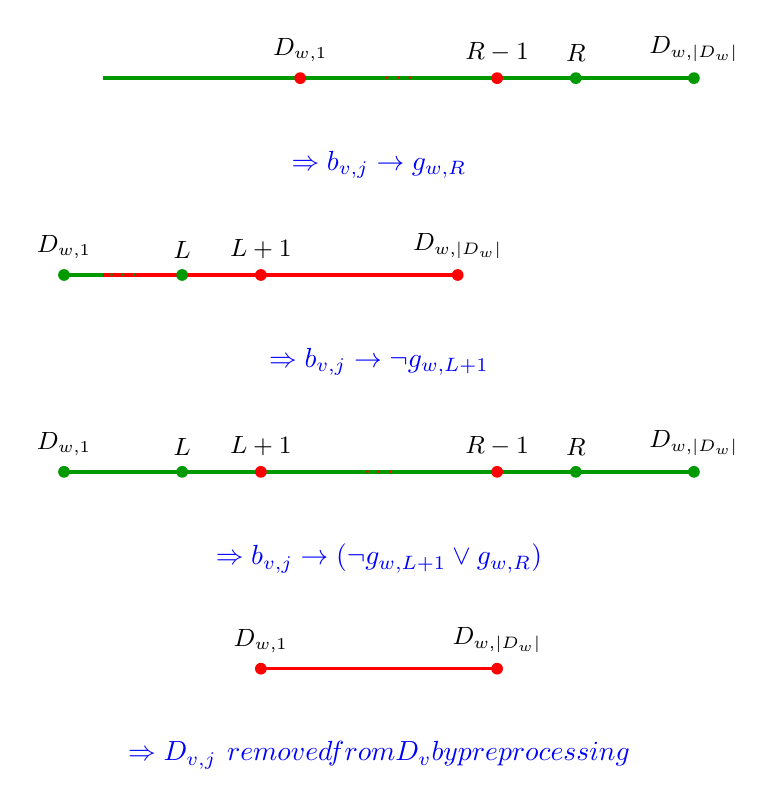
\begin{tikzpicture}[
    font=\small,
    axis/.style={-Latex, thick},
    forbidden/.style={fill=red!8},
    domain_invalid/.style={line width=1.2pt, red},
    domain_valid/.style={line width=1.2pt, green!60!black},
    domain_bound/.style={circle, fill, inner sep=1.5pt}
]

% ==========================================
% Case 1: D_w giao bên phải vùng cấm (eq:forbid_1)
\drawBase{7.5}{Case 1}
\draw[domain_invalid] (3.5, 7.8) -- (\fMax, 7.8);
\draw[domain_valid] (\fMax, 7.8) -- (8.5, 7.8);
\node[domain_bound, red, label=above:{$D_{w,1}$}] at (3.5, 7.8) {};
\node[red] at (4.75, 7.8) {$\dots$};
\node[domain_bound, red, label=above:{$R-1$}] at (6.0, 7.8) {};
\node[domain_bound, green!60!black, label=above:{$R$}] at (7.0, 7.8) {};
\node[green!60!black] at (7.75, 7.8) {$\dots$};
\node[domain_bound, green!60!black, label=above:{$D_{w,|D_w|}$}] at (8.5, 7.8) {};
% Đưa công thức xuống dưới trục tọa độ
\node[font=\bfseries, text=blue] at (4.5, 6.7) {$\Rightarrow b_{v,j} \rightarrow g_{w,R}$};

% ==========================================
% Case 2: D_w giao bên trái vùng cấm (eq:forbid_2)
\drawBase{5}{Case 2}
\draw[domain_valid] (0.5, 5.3) -- (\fMin, 5.3);
\draw[domain_invalid] (\fMin, 5.3) -- (5.5, 5.3);
\node[domain_bound, green!60!black, label=above:{$D_{w,1}$}] at (0.5, 5.3) {};
\node[green!60!black] at (1.25, 5.3) {$\dots$};
\node[domain_bound, green!60!black, label=above:{$L$}] at (2.0, 5.3) {};
\node[domain_bound, red, label=above:{$L+1$}] at (3.0, 5.3) {};
\node[red] at (4.25, 5.3) {$\dots$};
\node[domain_bound, red, label=above:{$D_{w,|D_w|}$}] at (5.5, 5.3) {};
% Đưa công thức xuống dưới trục tọa độ
\node[font=\bfseries, text=blue] at (4.5, 4.2) {$\Rightarrow b_{v,j} \rightarrow \neg g_{w,L+1}$};

% ==========================================
% Case 3: D_w trùm qua cả 2 bên vùng cấm (eq:forbid_3)
\drawBase{2.5}{Case 3}
\draw[domain_valid] (0.5, 2.8) -- (\fMin, 2.8);
\draw[domain_invalid] (\fMin, 2.8) -- (\fMax, 2.8);
\draw[domain_valid] (\fMax, 2.8) -- (8.5, 2.8);
\node[domain_bound, green!60!black, label=above:{$D_{w,1}$}] at (0.5, 2.8) {};
\node[green!60!black] at (1.25, 2.8) {$\dots$};
\node[domain_bound, green!60!black, label=above:{$L$}] at (2.0, 2.8) {};
\node[domain_bound, red, label=above:{$L+1$}] at (3.0, 2.8) {};
\node[red] at (4.5, 2.8) {$\dots$};
\node[domain_bound, red, label=above:{$R-1$}] at (6.0, 2.8) {};
\node[domain_bound, green!60!black, label=above:{$R$}] at (7.0, 2.8) {};
\node[green!60!black] at (7.75, 2.8) {$\dots$};
\node[domain_bound, green!60!black, label=above:{$D_{w,|D_w|}$}] at (8.5, 2.8) {};
% Đưa công thức xuống dưới trục tọa độ
\node[font=\bfseries, text=blue] at (4.5, 1.7) {$\Rightarrow b_{v,j} \rightarrow (\neg g_{w,L+1} \lor g_{w,R})$};

% ==========================================
% Case 4: no safe frequency remains; eliminated by preprocessing
\drawBase{0}{Case 4}
\draw[domain_invalid] (3.0, 0.3) -- (6.0, 0.3);
\node[domain_bound, red, label=above:{$D_{w,1}$}] at (3.0, 0.3) {};
\node[red] at (4.5, 0.3) {$\dots$};
\node[domain_bound, red, label=above:{$D_{w,|D_w|}$}] at (6.0, 0.3) {};
\node[font=\bfseries, text=blue] at (4.5, -0.8) {$\Rightarrow D_{v,j}\ \text{removed from }D_v\text{ by preprocessing}$};

\end{tikzpicture}%
}
\caption{Visualization of the four relative positions between the forbidden interval $[D_{v,j}-d_{vw},D_{v,j}+d_{vw}]$ and the domain $D_w$. Red segments denote forbidden frequencies of $w$, whereas green segments denote admissible frequencies. Cases 1--3 are encoded by the boundary implications in~\eqref{eq:forbid_1}--\eqref{eq:forbid_3}. In Case 4, all frequencies in $D_w$ are forbidden, so $D_{v,j}$ is removed from $D_v$ by preprocessing.}


\section{Proposed Exact Approach}
\label{sec:method}
This section details the proposed SAT-based methodology for solving the MO-FAP.
First, a domain preprocessing technique is applied to shrink the initial search space (Section~\ref{subsec:preprocessing}).
Next, we present a baseline Direct SAT Encoding (DSE) for the assignment, exact-distance, and interference constraints~\eqref{eq:ilp_domain},~\eqref{eq:ilp_exact}, and~\eqref{eq:ilp_ineq} (Section~\ref{subsec:sat_encoding}).
To overcome the combinatorial explosion inherent in the direct pairwise interference encoding, the Proposed Order-based SAT Encoding (POSE) is then introduced for the interference constraints (Section~\ref{subsec:order_encoding}).
Finally, the min-order objective~\eqref{eq:ilp_obj} is handled through active-frequency variables and an incremental SAT strategy (Section~\ref{subsec:incremental_sat}).

\subsection{Domain Preprocessing}
\label{subsec:preprocessing}
Before constructing the optimization models, the initial frequency domains are first simplified by an arc-consistency preprocessing step \cite{Aardal2007, Dib2009}. 
The purpose of this step is to remove a candidate frequency $f \in D_v$ whenever there exists an adjacent transmitter $w$ such that no frequency in $D_w$ can be paired with $f$ without violating the constraint on edge $vw$.
In addition, pre-assigned transmitters are handled by setting their domains to $D_v=\{p_v\}$, where $p_v$ is the prescribed frequency of transmitter $v$.
The output is a reduced set of domains, still denoted by $D_v$, which is used by the subsequent formulations and encodings.
If this preprocessing step makes some domain $D_v$ empty, then no feasible assignment can satisfy constraint~\eqref{eq:ilp_domain}, which requires each transmitter to be assigned exactly one frequency. Therefore, the instance is declared infeasible before any SAT or ILP model is constructed. In the subsequent formulations, each remaining domain $D_v$ is thus assumed to be nonempty.

For each edge $vw$, a candidate frequency $f \in D_v$ is retained only when there exists a frequency $h \in D_w$ that satisfies the corresponding edge constraint.
For interference constraints and bidirectional constraints, the corresponding domain filtering rules are defined in~\eqref{eq:pre_ineq} and~\eqref{eq:pre_eq}, respectively.

\begin{align}
    D_v &\leftarrow \{ f \in D_v \mid \exists h \in D_w : |f - h| > d_{vw} \},
    \notag \\
    &\quad \forall vw \in E_{ineq} \label{eq:pre_ineq} \\
    D_v &\leftarrow \{ f \in D_v \mid \exists h \in D_w : |f - h| = d_{vw} \},
    \notag \\
    &\quad \forall vw \in E_{eq} \label{eq:pre_eq}
\end{align}
 
Removing a frequency by the preprocessing rules does not remove any feasible solution of the original problem. Consider a transmitter-frequency pair $(v,f)$ with $f \in D_v$. 
If $f$ does not satisfy the retaining condition in either~\eqref{eq:pre_ineq} or~\eqref{eq:pre_eq} for an edge $vw$, then no frequency in $D_w$ can be assigned together with $f$ while satisfying the constraint on that edge. 
Therefore, $f$ cannot be assigned to $v$ in any feasible solution. It is thus safe to remove $f$ from $D_v$ before constructing the optimization models.
\subsection{Direct SAT Encoding}
\label{subsec:sat_encoding}

Unlike the ILP formulation, our SAT encoding relies on the positional order of the candidate frequencies. We define a Boolean variable $b_{v,j} = \text{True}$ if and only if transmitter $v$ is assigned the $j$-th frequency in its preprocessed domain $D_v$ (sorted in ascending order). Let $D_{v,j}$ denote the actual frequency value at index $j$. Based on this notation, the baseline feasibility constraints are encoded into three logical formulations, expressed in~\eqref{eq:sat_domain}--\eqref{eq:sat_ineq}.

% Equation~\eqref{eq:sat_domain} represents the Exactly-One constraint. 
% Although expressed in this numerical form for mathematical clarity, it can be seamlessly translated into standard Conjunctive Normal Form (CNF) clauses using well-established cardinality encoding schemes (e.g., pairwise AMO and ALO) readily supported by modern SAT libraries \cite{imms-sat18, itk-sat24}. 
Equation~\eqref{eq:sat_domain} encodes the Exactly-One constraint. Although written in a numerical form for clarity, it can be translated into Conjunctive Normal Form (CNF) using standard cardinality encodings (e.g., At-Most-One and At-Least-One), which are readily supported by modern SAT libraries \cite{imms-sat18, itk-sat24}.
Notably, no additional clauses are required to handle the pre-assignment constraint. Since the preprocessed domain of any pre-assigned transmitter naturally contains exactly one element ($|D_v| = 1$),~\eqref{eq:sat_domain} inherently reduces to $b_{v,1} = \text{True}$, natively satisfying the condition. 
Bidirectional constraints are expressed in~\eqref{eq:sat_exact}: if transmitter $v$ is assigned the $j$-th frequency, the paired transmitter $w$ must be assigned a frequency index $j'$ such that the frequency separation between their actual values is exactly $d_{vw}$, and vice versa. 
Finally, interference constraints (which correspond to the binary packing constraints in the ILP model) are handled in~\eqref{eq:sat_ineq} via conflict clauses: if transmitter $v$ selects the frequency index $j$, then the adjacent transmitter $w$ is strictly prohibited from adopting any frequency index $j'$ whose separation is less than or equal to the safety threshold $d_{vw}$.
 \begin{align}
    & \sum_{j=1}^{|D_v|} b_{v,j} = 1, \quad \forall v \in V \label{eq:sat_domain} \\
    & b_{v,j} \rightarrow \bigvee_{j'} b_{w,j'}, \notag \\
    & \quad \forall vw \in E_{eq}, \; \forall j \in \{1, \dots, |D_v|\}, \notag \\
    & \quad \forall j' \in \{1, \dots, |D_w|\} : |D_{v,j} - D_{w,j'}| = d_{vw} \label{eq:sat_exact} \\
    & \neg b_{v,j} \vee \neg b_{w,j'}, \notag \\
    & \quad \forall vw \in E_{ineq}, \; \forall j \in \{1, \dots, |D_v|\}, \notag \\
    & \quad \forall j' \in \{1, \dots, |D_w|\} : |D_{v,j} - D_{w,j'}| \le d_{vw} \label{eq:sat_ineq}
\end{align}

Thus, the Boolean variables $b_{v,j}$ and constraints~\eqref{eq:sat_domain}--\eqref{eq:sat_ineq} ensure that every satisfying assignment of the DSE formula corresponds to a feasible frequency assignment satisfying constraints~\eqref{eq:ilp_domain},~\eqref{eq:ilp_exact}, and~\eqref{eq:ilp_ineq}. Conversely, any frequency assignment satisfying these constraints can be translated into a satisfying assignment of the DSE formula. This correctness property is formalized in Proposition~\ref{prop:dse_correctness}.

\begin{proposition}
\label{prop:dse_correctness}
For the preprocessed domains, every satisfying assignment of the DSE constraints~\eqref{eq:sat_domain}--\eqref{eq:sat_ineq} induces a frequency assignment satisfying constraints~\eqref{eq:ilp_domain},~\eqref{eq:ilp_exact}, and~\eqref{eq:ilp_ineq}. Conversely, every frequency assignment satisfying these constraints induces a satisfying assignment of the DSE constraints.
\end{proposition}

\begin{IEEEproof}
Consider the direct mapping in which $b_{v,j}$ is true exactly when transmitter $v$ is assigned frequency $D_{v,j}$ ($x_{v,D_{v,j}}=1$ in the ILP formulation).
Suppose first that the DSE constraints have a satisfying assignment. By~\eqref{eq:sat_domain}, exactly one $b_{v,j}$ is true for each transmitter $v$, so the induced frequency assignment selects exactly one frequency for each transmitter and satisfies~\eqref{eq:ilp_domain}. For every edge $vw\in E_{eq}$, constraint~\eqref{eq:sat_exact} states that once $v$ selects $D_{v,j}$, transmitter $w$ must select one of the frequencies $D_{w,j'}$ whose distance from $D_{v,j}$ is exactly $d_{vw}$. Therefore, the selected pair on edge $vw$ satisfies~\eqref{eq:ilp_exact}. For every edge $vw\in E_{ineq}$, constraint~\eqref{eq:sat_ineq} adds a conflict clause for each pair with $|D_{v,j}-D_{w,j'}|\le d_{vw}$, preventing both variables in any such pair from being true simultaneously. Hence, every selected pair has distance greater than $d_{vw}$, so~\eqref{eq:ilp_ineq} holds.

Conversely, let a frequency assignment satisfy~\eqref{eq:ilp_domain},~\eqref{eq:ilp_exact}, and~\eqref{eq:ilp_ineq}. 
For each transmitter $v$, let $j$ be the index such that the assigned frequency of $v$ is $D_{v,j}$.
The corresponding assignment of the DSE variables sets $b_{v,j}$ to true and sets $b_{v,k}$ to false for all $k\neq j$.
Since the assignment selects exactly one frequency for each transmitter, the DSE exactly-one constraint~\eqref{eq:sat_domain} is satisfied.
For every exact-distance edge $vw\in E_{eq}$, constraint~\eqref{eq:ilp_exact} forbids all pairs whose distance is not $d_{vw}$. Therefore, if a pair is selected by the frequency assignment, its distance must be exactly $d_{vw}$, and the corresponding implication in~\eqref{eq:sat_exact} is satisfied.
Similarly, for every interference edge $vw\in E_{ineq}$, constraint~\eqref{eq:ilp_ineq} forbids all pairs whose distance is at most $d_{vw}$. Therefore, no forbidden pair in~\eqref{eq:sat_ineq} is selected simultaneously. Hence, all DSE constraints are satisfied.
\end{IEEEproof}
\subsection{Proposed Order-Based SAT Encoding}
\label{subsec:order_encoding}
Although DSE provides an intuitive formulation, expressing the interference constraints~\eqref{eq:sat_ineq} in this manner may require many clauses, since each forbidden frequency pair is encoded separately.
To overcome this limitation, POSE uses order variables following order encoding~\cite{Crawford1994Scheduling,Tamura2009OrderEncoding,Petke2011Order_encoding,Abio2014LinearSAT} to reformulate the MO-FAP interference constraints without encoding each forbidden frequency pair separately.
Note that this work does not introduce a new order encoding.
The main contribution of POSE is the adaptation of order variables to the interference constraints of MO-FAP. It links these variables with $b_{v,j}$ and uses the resulting representation to encode forbidden frequency intervals as an alternative to the pairwise formulation used in DSE.

Specifically, while retaining the Boolean variables $b_{v,j}$ and the preprocessed domain $D_v$, POSE introduces a supplementary set of Boolean variables, denoted by $g_{v,j}$.
The domain $D_v$ is sorted in increasing order, and $g_{v,j}$ represents whether the selected frequency index of vertex $v$ is greater than or equal to $j$.
The variables $b_{v,j}$ and $g_{v,j}$ are linked by constraints~\eqref{eq:g_b_connect}--\eqref{eq:g_propagation}, where $|D_v|$ denotes the number of candidate frequencies in the domain of vertex $v$.
These constraints also enforce that exactly one frequency index is selected for each transmitter.
Lemma~\ref{lem:order_variable_semantics} formalizes this relationship between the selected $b$ variable and the corresponding $g$ variables.
\begin{align}
    & b_{v,j} \leftrightarrow g_{v,j} \wedge \neg g_{v,j+1}, \forall v \in V, \forall j \in \{1, \dots, |D_v|-1\} \label{eq:g_b_connect} \\
    & b_{v,|D_v|} \leftrightarrow g_{v,|D_v|}, \quad \forall v \in V \label{eq:g_right_bound} \\
    & g_{v,1}, \quad \forall v \in V \label{eq:g_left_bound} \\
    & g_{v,j} \rightarrow g_{v,j-1}, \quad \forall v \in V, \forall j \in \{2, \dots, |D_v|\} \label{eq:g_propagation}
\end{align}

\begin{lemma}
\label{lem:order_variable_semantics}
For each transmitter $v$, constraints~\eqref{eq:g_b_connect}--\eqref{eq:g_propagation} enforce exactly one true variable among $\{b_{v,j}\mid j\in\{1,\ldots,|D_v|\}\}$. If $b_{v,t}$ is this true variable, then $g_{v,j}$ is true if and only if the selected frequency index $t$ is greater than or equal to $j$ in the sorted domain $D_v$.
\end{lemma}
\begin{IEEEproof}
Let $n=|D_v|$ and consider any assignment satisfying~\eqref{eq:g_b_connect}--\eqref{eq:g_propagation}. By~\eqref{eq:g_left_bound}, $g_{v,1}$ is true. Constraint~\eqref{eq:g_propagation} implies that if $g_{v,j}$ is true, then all variables $g_{v,k}$ with $k<j$ are also true. Therefore, the true $g$ variables form a nonempty prefix of the ordered domain.

First, suppose that there exists an index $r$ such that $g_{v,r}$ is false, and let $r$ be the smallest such index. Then $r>1$. Set $t=r-1$. By the choice of $r$, $g_{v,t}$ is true and $g_{v,t+1}$ is false. Substituting $j=t$ into~\eqref{eq:g_b_connect} gives $b_{v,t}\leftrightarrow(g_{v,t}\wedge\neg g_{v,t+1})$, so $b_{v,t}$ is true.
For any $k<t$, $g_{v,k+1}$ is true, so~\eqref{eq:g_b_connect} makes $b_{v,k}$ false. For any $t<k<n$, $g_{v,k}$ is false, so~\eqref{eq:g_b_connect} also makes $b_{v,k}$ false. Since $g_{v,n}$ is false in this case,~\eqref{eq:g_right_bound} makes $b_{v,n}$ false. Hence, exactly one $b$ variable is true, namely $b_{v,t}$. Moreover, $g_{v,j}$ is true exactly for the indices $j\le t$, which is equivalent to $t\ge j$.

It remains to consider the case in which no $g_{v,j}$ is false. Then all variables $g_{v,j}$ are true. By~\eqref{eq:g_right_bound}, $b_{v,n}$ is true. For every $k<n$, $g_{v,k+1}$ is true, so~\eqref{eq:g_b_connect} makes $b_{v,k}$ false. Hence, exactly one $b$ variable is true, namely $b_{v,n}$. In this case the selected index is $t=n$, and $g_{v,j}$ is true for every valid index $j$, which is equivalent to $t\ge j$.
\end{IEEEproof}

Subsequently, the order variables $g$ are used to reformulate the interference constraints. When transmitter $v$ is assigned the frequency $D_{v,j}$ (i.e., $b_{v,j}=\text{True}$), it induces the forbidden interval $[D_{v,j}-d_{vw},\,D_{v,j}+d_{vw}]$ for its adjacent transmitter $w$. Figure~\ref{fig:domain_pruning_cases} illustrates the relative positions between this forbidden interval and the preprocessed domain $D_w$, which is nonempty at this stage. Three situations may then arise. In Cases~1 and Case~2, the domain $D_w$ lies entirely outside the forbidden interval, either to its left or to its right. In this situation, every value in $D_w$ already satisfies the interference constraint, so no additional constraint is required. In Cases~3, Case~4, and Case~5, the domain $D_w$ overlaps the forbidden interval on the left, on both sides, or on the right. In these cases, the remaining values of $D_w$ outside the forbidden interval must be characterized explicitly. In Case~6, all values in $D_w$ fall inside the forbidden interval. Consequently, $D_{v,j}$ has no compatible value in $D_w$ and is therefore removed from $D_v$ during preprocessing.
\begin{figure}[]
\centering

% Đưa toàn bộ việc định nghĩa macro ra NGOÀI lệnh \resizebox
\def\xCenter{4.5}
\def\d{2}
\def\fMin{\xCenter-\d} % 2.5
\def\fMax{\xCenter+\d} % 6.5

\newcommand{\drawBase}[2]{
    % Vùng cấm màu đỏ
    \fill[forbidden] (\fMin, #1-0.3) rectangle (\fMax, #1+0.7);
    \draw[red, dashed, thick] (\fMin, #1-0.3) -- (\fMin, #1+0.7);
    \draw[red, dashed, thick] (\fMax, #1-0.3) -- (\fMax, #1+0.7);

    % Trục f vẽ sau để nổi lên trên
    \draw[axis] (0, #1) -- (9.5, #1) node[right] {$f \in D$};

    % Đánh dấu tâm D_{v,j} và giới hạn
    \draw[thick] (\xCenter, #1-0.1) -- (\xCenter, #1+0.1);
    \node[below, font=\footnotesize] at (\xCenter, #1) {$D_{v,j}$};
    \node[red, below, font=\footnotesize] at (\fMin, #1) {$D_{v,j}-d_{vw}$};
    \node[red, below, font=\footnotesize] at (\fMax, #1) {$D_{v,j}+d_{vw}$};

    % Tên Case
    \node[left, font=\bfseries] at (-0.5, #1+0.3) {#2};
}

\iffalse
\fi
\resizebox{\columnwidth}{!}{%
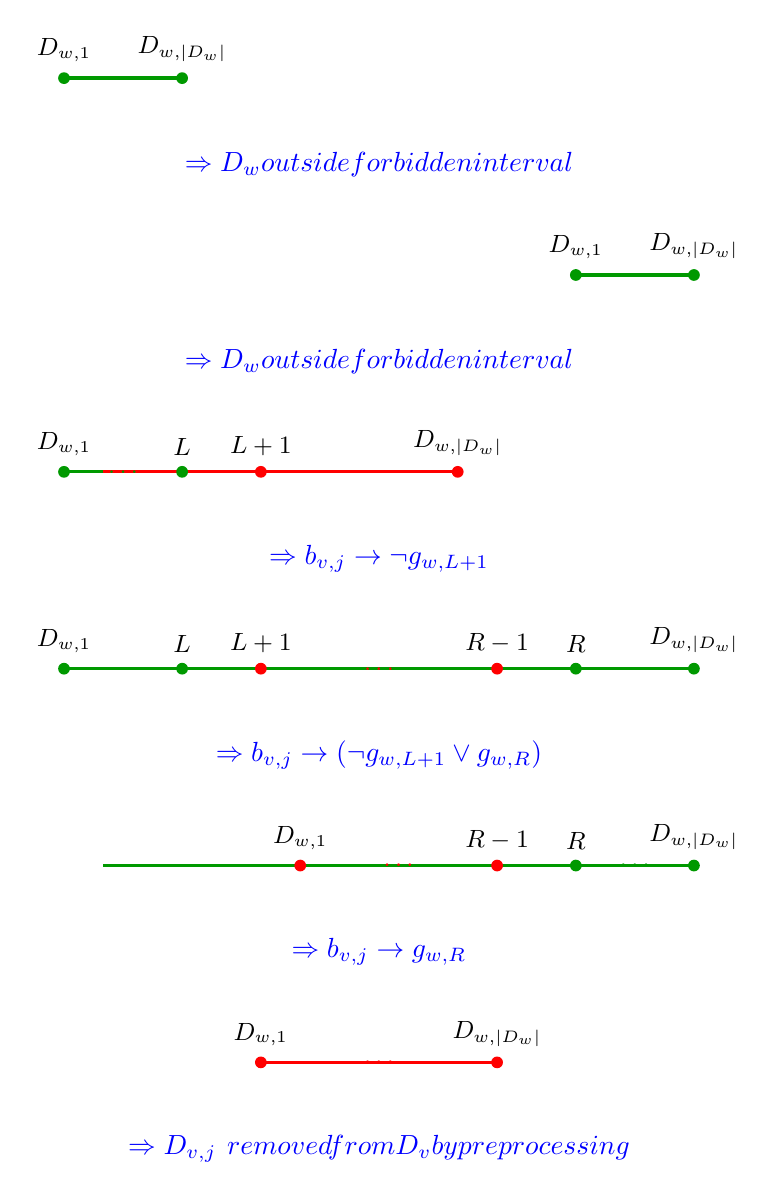
\begin{tikzpicture}[
    font=\small,
    axis/.style={-Latex, thick},
    forbidden/.style={fill=red!8},
    domain_invalid/.style={line width=1.2pt, red},
    domain_valid/.style={line width=1.2pt, green!60!black},
    domain_bound/.style={circle, fill, inner sep=1.5pt}
]

% ==========================================
% Case 1: D_w lies entirely to the left of the forbidden interval
\drawBase{12.5}{Case 1}
\draw[domain_valid] (0.5, 12.8) -- (2.0, 12.8);
\node[domain_bound, green!60!black, label=above:{$D_{w,1}$}] at (0.5, 12.8) {};
\node[green!60!black] at (1.25, 12.8) {$\dots$};
\node[domain_bound, green!60!black, label=above:{$D_{w,|D_w|}$}] at (2.0, 12.8) {};
\node[font=\bfseries, text=blue] at (4.5, 11.7) {$\Rightarrow D_w \text{ outside forbidden interval}$};

% ==========================================
% Case 2: D_w lies entirely to the right of the forbidden interval
\drawBase{10}{Case 2}
\draw[domain_valid] (7.0, 10.3) -- (8.5, 10.3);
\node[domain_bound, green!60!black, label=above:{$D_{w,1}$}] at (7.0, 10.3) {};
\node[green!60!black] at (7.75, 10.3) {$\dots$};
\node[domain_bound, green!60!black, label=above:{$D_{w,|D_w|}$}] at (8.5, 10.3) {};
\node[font=\bfseries, text=blue] at (4.5, 9.2) {$\Rightarrow D_w \text{ outside forbidden interval}$};

% ==========================================
% Case 3: D_w overlaps the forbidden interval on the left
\drawBase{7.5}{Case 3}
\draw[domain_valid] (0.5, 7.8) -- (\fMin, 7.8);
\draw[domain_invalid] (\fMin, 7.8) -- (5.5, 7.8);
\node[domain_bound, green!60!black, label=above:{$D_{w,1}$}] at (0.5, 7.8) {};
\node[green!60!black] at (1.25, 7.8) {$\dots$};
\node[domain_bound, green!60!black, label=above:{$L$}] at (2.0, 7.8) {};
\node[domain_bound, red, label=above:{$L+1$}] at (3.0, 7.8) {};
\node[red] at (4.25, 7.8) {$\dots$};
\node[domain_bound, red, label=above:{$D_{w,|D_w|}$}] at (5.5, 7.8) {};
\node[font=\bfseries, text=blue] at (4.5, 6.7) {$\Rightarrow b_{v,j} \rightarrow \neg g_{w,L+1}$};

% ==========================================
% Case 4: D_w extends on both sides of the forbidden interval
\drawBase{5}{Case 4}
\draw[domain_valid] (0.5, 5.3) -- (\fMin, 5.3);
\draw[domain_invalid] (\fMin, 5.3) -- (\fMax, 5.3);
\draw[domain_valid] (\fMax, 5.3) -- (8.5, 5.3);
\node[domain_bound, green!60!black, label=above:{$D_{w,1}$}] at (0.5, 5.3) {};
\node[green!60!black] at (1.25, 5.3) {$\dots$};
\node[domain_bound, green!60!black, label=above:{$L$}] at (2.0, 5.3) {};
\node[domain_bound, red, label=above:{$L+1$}] at (3.0, 5.3) {};
\node[red] at (4.5, 5.3) {$\dots$};
\node[domain_bound, red, label=above:{$R-1$}] at (6.0, 5.3) {};
\node[domain_bound, green!60!black, label=above:{$R$}] at (7.0, 5.3) {};
\node[green!60!black] at (7.75, 5.3) {$\dots$};
\node[domain_bound, green!60!black, label=above:{$D_{w,|D_w|}$}] at (8.5, 5.3) {};
\node[font=\bfseries, text=blue] at (4.5, 4.2) {$\Rightarrow b_{v,j} \rightarrow (\neg g_{w,L+1} \lor g_{w,R})$};

% ==========================================
% Case 5: D_w overlaps the forbidden interval on the right
\drawBase{2.5}{Case 5}
\draw[domain_invalid] (3.5, 2.8) -- (\fMax, 2.8);
\draw[domain_valid] (\fMax, 2.8) -- (8.5, 2.8);
\node[domain_bound, red, label=above:{$D_{w,1}$}] at (3.5, 2.8) {};
\node[red] at (4.75, 2.8) {$\dots$};
\node[domain_bound, red, label=above:{$R-1$}] at (6.0, 2.8) {};
\node[domain_bound, green!60!black, label=above:{$R$}] at (7.0, 2.8) {};
\node[green!60!black] at (7.75, 2.8) {$\dots$};
\node[domain_bound, green!60!black, label=above:{$D_{w,|D_w|}$}] at (8.5, 2.8) {};
\node[font=\bfseries, text=blue] at (4.5, 1.7) {$\Rightarrow b_{v,j} \rightarrow g_{w,R}$};

% ==========================================
% Case 6: no safe frequency remains; eliminated by preprocessing
\drawBase{0}{Case 6}
\draw[domain_invalid] (3.0, 0.3) -- (6.0, 0.3);
\node[domain_bound, red, label=above:{$D_{w,1}$}] at (3.0, 0.3) {};
\node[red] at (4.5, 0.3) {$\dots$};
\node[domain_bound, red, label=above:{$D_{w,|D_w|}$}] at (6.0, 0.3) {};
\node[font=\bfseries, text=blue] at (4.5, -0.8) {$\Rightarrow D_{v,j}\ \text{removed from }D_v\text{ by preprocessing}$};

\end{tikzpicture}%
}
\caption{Relative positions between the forbidden interval $[D_{v,j}-d_{vw},D_{v,j}+d_{vw}]$ and the domain $D_w$. Red segments denote forbidden values in $D_w$, and green segments denote the remaining values in $D_w$.}
\label{fig:domain_pruning_cases}
\end{figure}

In Cases~1 and~2, the domain $D_w$ lies entirely outside the forbidden interval. Therefore, every value in $D_w$ already satisfies the interference constraint, and no additional constraint is required. 
% For the remaining cases, the corresponding clauses are constructed by~\eqref{eq:forbid_1}--\eqref{eq:forbid_3}. 
For Cases~3--5, in which at least one value of $D_w$ lies in the forbidden interval, the corresponding clauses are constructed by~\eqref{eq:forbid_1}--\eqref{eq:forbid_3}.
In Case~3, the forbidden interval overlaps the right part of $D_w$, so the remaining values of $D_w$ lie entirely to the left of the forbidden interval, and the clause is given by~\eqref{eq:forbid_2}. In Case~4, the forbidden interval lies strictly inside $D_w$, so the remaining values of $D_w$ appear on both sides of the forbidden interval, and the clause is given by~\eqref{eq:forbid_3}. In Case~5, the forbidden interval overlaps the left part of $D_w$, so the remaining values of $D_w$ lie entirely to the right of the forbidden interval, and the clause is given by~\eqref{eq:forbid_1}. Notably, $L$ is used only in~\eqref{eq:forbid_2} and~\eqref{eq:forbid_3}, whereas $R$ is used only in~\eqref{eq:forbid_3} and~\eqref{eq:forbid_1}. Therefore, each boundary index is defined only in the cases where the corresponding side of $D_w$ exists.

\begin{align}
    b_{v,j} &\rightarrow \neg g_{w,L+1} \label{eq:forbid_2} \\
    b_{v,j} &\rightarrow (\neg g_{w,L+1} \lor g_{w,R}) \label{eq:forbid_3} \\
    b_{v,j} &\rightarrow g_{w,R} \label{eq:forbid_1} \\
    &\text{where } L = \operatorname{arg\,max}\limits_{k} \{ k \mid D_{w,k} < D_{v,j} - d_{vw} \} \notag \\
    &\phantom{\text{where }} R = \operatorname{arg\,min}\limits_{k} \{ k \mid D_{w,k} > D_{v,j} + d_{vw} \} \notag
\end{align}

Case~6 occurs when every value in $D_w$ lies in the forbidden interval induced by $D_{v,j}$. In the current formulation, this case is eliminated by preprocessing, whereas without preprocessing it can be encoded directly by the unary clause $\neg b_{v,j}$. Proposition~\ref{prop:pose_correctness} shows that these boundary clauses are equivalent to the pairwise interference clauses of DSE.

\begin{proposition}
\label{prop:pose_correctness}
For the preprocessed domains, POSE ensures that each transmitter is assigned exactly one frequency. More precisely, constraints~\eqref{eq:g_b_connect}--\eqref{eq:g_propagation} are equivalent to the DSE constraint~\eqref{eq:sat_domain}.
Under these constraints,~\eqref{eq:forbid_2} in Case~3,~\eqref{eq:forbid_3} in Case~4, and~\eqref{eq:forbid_1} in Case~5 are satisfied if and only if the assignment to the variables $b$ satisfies the DSE interference constraints~\eqref{eq:sat_ineq}. 
POSE uses the same exact-distance constraints~\eqref{eq:sat_exact} as DSE. 
Therefore, Proposition~\ref{prop:dse_correctness} implies that POSE represents exactly the frequency assignments satisfying constraints~\eqref{eq:ilp_domain},~\eqref{eq:ilp_exact}, and~\eqref{eq:ilp_ineq}.
\end{proposition}
\begin{IEEEproof}
By Lemma~\ref{lem:order_variable_semantics}, every assignment satisfying constraints~\eqref{eq:g_b_connect}--\eqref{eq:g_propagation} has exactly one true variable $b_{v,t}$ for each transmitter $v$. Conversely, suppose that~\eqref{eq:sat_domain} holds and $b_{v,t}$ is the unique true variable for transmitter $v$. Set $g_{v,k}$ to true if and only if $t\ge k$. This assignment satisfies constraints~\eqref{eq:g_b_connect}--\eqref{eq:g_propagation}. Hence, these constraints are equivalent to~\eqref{eq:sat_domain}.

Consider an interference edge $vw\in E_{ineq}$ and an index $j\in\{1,\ldots,|D_v|\}$ such that $b_{v,j}$ is true. Let $b_{w,t}$ be the unique true variable for transmitter $w$. By Lemma~\ref{lem:order_variable_semantics}, $g_{w,k}$ is true if and only if $t\ge k$.

In Case~3, constraint~\eqref{eq:forbid_2} requires $\neg g_{w,L+1}$ because $b_{v,j}$ is true. By Lemma~\ref{lem:order_variable_semantics}, $g_{w,L+1}$ is true if and only if $t\ge L+1$. Therefore, $\neg g_{w,L+1}$ is equivalent to $t\le L$. Since $D_w$ is sorted and $L$ is the largest index satisfying $D_{w,L}<D_{v,j}-d_{vw}$, the selected frequency $D_{w,t}$ lies to the left of the forbidden interval.
For each $k\in\{L+1,\ldots,|D_w|\}$, DSE includes the clause $\neg b_{v,j}\lor\neg b_{w,k}$ in~\eqref{eq:sat_ineq}. Since $b_{v,j}$ is true, these clauses force $b_{w,L+1},\ldots,b_{w,|D_w|}$ to be false. Hence, the unique true variable $b_{w,t}$ must satisfy $t\le L$. DSE therefore imposes the same restriction as~\eqref{eq:forbid_2}.

In Case~5, constraint~\eqref{eq:forbid_1} requires $g_{w,R}$ because $b_{v,j}$ is true. By Lemma~\ref{lem:order_variable_semantics}, this condition is equivalent to $t\ge R$. Since $D_w$ is sorted and $R$ is the smallest index satisfying $D_{w,R}>D_{v,j}+d_{vw}$, the selected frequency $D_{w,t}$ lies to the right of the forbidden interval.
For each $k\in\{1,\ldots,R-1\}$, DSE includes the clause $\neg b_{v,j}\lor\neg b_{w,k}$ in~\eqref{eq:sat_ineq}. Since $b_{v,j}$ is true, these clauses force $b_{w,1},\ldots,b_{w,R-1}$ to be false. Hence, the unique true variable $b_{w,t}$ must satisfy $t\ge R$. DSE therefore imposes the same restriction as~\eqref{eq:forbid_1}.

Case~4 combines the two possibilities established in Cases~3 and~5. When $b_{v,j}$ is true, constraint~\eqref{eq:forbid_3} requires $\neg g_{w,L+1}\lor g_{w,R}$, which is equivalent to $t\le L$ or $t\ge R$. DSE includes the clause $\neg b_{v,j}\lor\neg b_{w,k}$ for each $k\in\{L+1,\ldots,R-1\}$ in~\eqref{eq:sat_ineq}. Since $b_{v,j}$ is true, these clauses force $b_{w,L+1},\ldots,b_{w,R-1}$ to be false. Hence, the unique true variable $b_{w,t}$ must satisfy either $t\le L$ or $t\ge R$. DSE therefore imposes the same restriction as~\eqref{eq:forbid_3}.

In each case, the POSE constraint and the corresponding DSE clauses are equivalent to the same condition on the selected index $t$. Therefore, the equivalence holds in both directions.
Cases~1 and~2 require no additional constraints, while Case~6 cannot occur in the preprocessed domains. If $b_{v,j}$ is false, frequency $D_{v,j}$ is not selected, and neither encoding restricts transmitter $w$ based on this frequency. Therefore, over every interference edge $vw\in E_{ineq}$ and every index $j\in\{1,\ldots,|D_v|\}$, constraints~\eqref{eq:forbid_1}--\eqref{eq:forbid_3} exclude exactly the same assignments as~\eqref{eq:sat_ineq}. Together with the equivalence between constraints~\eqref{eq:g_b_connect}--\eqref{eq:g_propagation} and~\eqref{eq:sat_domain}, and the unchanged exact-distance constraints~\eqref{eq:sat_exact}, this establishes the result by Proposition~\ref{prop:dse_correctness}.In each case, the POSE constraint and the corresponding DSE clauses are equivalent to the same condition on the selected index $t$. Therefore, the equivalence holds in both directions.
\end{IEEEproof}

\subsection{Objective Function Optimization via Incremental SAT}
\label{subsec:incremental_sat}
After the hard constraints of the MO-FAP in \eqref{eq:ilp_domain}--\eqref{eq:ilp_ineq} have been encoded, the remaining task is to minimize the total number of distinct frequencies utilized. Let $D_m$ denote the frequency value at the $m$-th position of the sorted global domain $D$, where $1 \le m \le N=|D|$.

% We introduce Boolean variables $A_m$, where $A_m=\text{True}$ is activated when the frequency $D_m$ is used by at least one transmitter. 
We introduce Boolean variables $A_m$, where $A_m$ is set to $\text{True}$ whenever the frequency $D_m$ is used by at least one transmitter.
The connection between the local assignment variables $b_{v,j}$ and the global frequency-usage variables $A_m$ is expressed by~\eqref{eq:active_link}.
As illustrated in Fig.~\ref{fig:b_to_A_implication}, each selected local assignment $b_{v,j}$ activates the corresponding global usage variable $A_m$, and the set of active $A_m$ variables is then minimized by the objective encoding.


\begin{align}
    b_{v,j} \rightarrow A_m, \quad \forall v \in V,\; \forall j,m : D_{v,j} = D_m.
    \label{eq:active_link}
\end{align}

\begin{figure}[!htbp]
\centering
\resizebox{\columnwidth}{!}{%
\begin{tikzpicture}[
    node distance = 1.5cm and 1cm,
    var_box/.style = {draw, rectangle, minimum width=1.2cm, minimum height=0.8cm, align=center, font=\small},
    active_u/.style = {var_box, draw=blue, fill=blue!15, font=\small\bfseries},
    inactive_u/.style = {var_box, draw=blue!50, fill=blue!5, text=gray},
    arrow_u/.style = {-Latex, thick, blue},
    active_v/.style = {var_box, draw=red, fill=red!15, font=\small\bfseries},
    inactive_v/.style = {var_box, draw=red!50, fill=red!5, text=gray},
    arrow_v/.style = {-Latex, thick, red},
    active_A/.style = {var_box, draw=green!60!black, fill=green!15, font=\small\bfseries},
    inactive_A/.style = {var_box, draw=gray, fill=gray!10, text=gray},
    arrow_A/.style = {-Latex, thick, green!60!black}
]

% --- Local Domains ---
\node[text=blue] (u_label) at (-1.5, 2.2) {\textbf{Transmitter $u$}};
\node[inactive_u] (xu1) at (-3, 1) {$b_{u,1}$\\($f=10$)};
\node[active_u] (xu2) at (-1.5, 1) {$b_{u,2}$\\($f=20$)}; 
\node[inactive_u] (xu3) at (0, 1) {$b_{u,3}$\\($f=30$)};

\node[text=red] (v_label) at (4, 2.2) {\textbf{Transmitter $v$}};
\node[inactive_v] (xv1) at (2.5, 1) {$b_{v,1}$\\($f=20$)};
\node[inactive_v] (xv2) at (4, 1) {$b_{v,2}$\\($f=30$)};
\node[active_v] (xv3) at (5.5, 1) {$b_{v,3}$\\($f=40$)}; 

% --- Global Frequency Pool ---
\node (global_label) at (-4, -1) {\textbf{Global Domain ($D$)}};
\node[inactive_A] (A1) at (-1, -1.8) {$A_1$\\($f=10$)};
\node[active_A] (A2) at (0.5, -1.8) {$A_2$\\($f=20$)};
\node[inactive_A] (A3) at (2, -1.8) {$A_3$\\($f=30$)};
\node[active_A] (A4) at (3.5, -1.8) {$A_4$\\($f=40$)};

% --- Implications ---
\draw[-Latex, draw=blue!30] (xu1.south) -- (A1.north);
\draw[arrow_u] (xu2.south) -- node[left, pos=0.5, font=\footnotesize, fill=white, inner sep=1pt] {$b_{u,2} \rightarrow A_2$} (A2.north);
\draw[-Latex, draw=blue!30] (xu3.south) -- (A3.north);

\draw[-Latex, draw=red!30] (xv1.south) -- (A2.north);
\draw[-Latex, draw=red!30] (xv2.south) -- (A3.north);
\draw[arrow_v] (xv3.south) -- node[right, pos=0.4, font=\footnotesize, fill=white, inner sep=1pt] {$b_{v,3} \rightarrow A_4$} (A4.north);

% --- Sequential Counter ---
\node[draw=green!60!black, rectangle, minimum width=6cm, minimum height=1cm, fill=green!5, font=\bfseries] (counter) at (1.25, -4) {\textbf{Minimum Order} \small (Minimizing $\sum A_{m}$)};

% Arrows to Counter
\draw[-Latex, draw=gray!50] (A1.south) -- (A1.south |- counter.north);
\draw[arrow_A] (A2.south) -- (A2.south |- counter.north);
\draw[-Latex, draw=gray!50] (A3.south) -- (A3.south |- counter.north);
\draw[arrow_A] (A4.south) -- (A4.south |- counter.north);

\end{tikzpicture}%
}
\caption{Mapping from local assignment variables ($b_{v,j}$) to global frequency-usage variables ($A_m$).}
\label{fig:b_to_A_implication}
\end{figure}

The optimization of the objective function is performed by a linear search over the number of active frequencies. The solver first finds a feasible assignment and uses its number of distinct frequencies as the initial upper bound $UB$. It then searches for a better solution satisfying an At-Most-$k$ constraint with $k=UB-1$. Whenever such a solution is found, $UB$ is updated and the bound is tightened again. When the solver returns \texttt{UNSAT}, the last feasible bound is certified as globally optimal.

These search iterations could be executed as independent SAT calls, where each new value of $k$ requires constructing a new At-Most-$k$ constraint and solving a fresh formula. However, this strategy discards the learned clauses obtained in previous iterations. Therefore, we use the incremental solving mechanism supported by PySAT \cite{imms-sat18,itk-sat24}. In the baseline incremental strategy, denoted as INC, the At-Most-$k$ constraints are handled by \texttt{ITotalizer} \cite{martins2014incremental,Bailleux2003}, which exposes bound literals that can be passed as assumptions to tighten the cardinality limit across iterations. This allows INC to reuse the same solver instance instead of rebuilding the entire SAT formula for every value of $k$.

Although INC supports learned-clause reuse through assumptions, its Totalizer-based objective encoding introduces considerable structural overhead. To reduce this overhead, we propose INCSC, an Incremental SAT strategy that keeps the same assumptions-based optimization loop as INC but replaces the Totalizer with a Sequential Counter encoding \cite{Sinz2005}. The Sequential Counter encoding is generated only once for the initial bound $K=UB-1$. 
For the ordered sequence of global usage variables $A_1,\dots,A_N$, INCSC introduces auxiliary variables $S_{i,c}$, where $1 \le i \le N$ and $1 \le c \le \min(i,K)$. The variable $S_{i,c}$ is true if and only if at least $c$ variables among $A_1,\dots,A_i$ are true. Equivalently, each prefix state $S_i$ is a vector of $\min(i,K)$ bits, $S_i=(S_{i,1},\dots,S_{i,\min(i,K)})$: $S_1$ has one bit, $S_2$ has two bits, and for $i \ge K$, $S_i$ has $K$ bits. This semantics is enforced by the constraints in~\eqref{eq:nsc_1}--\eqref{eq:nsc_7}. As a result, INCSC reduces the objective encoding to $\mathcal{O}(NK)$ auxiliary variables and clauses, compared with the $\mathcal{O}(N \log N)$ auxiliary variables and $\mathcal{O}(N^2)$ clauses required by INC.

\begin{align}
    & \bigwedge_{i=1}^{N} \left( A_i \rightarrow S_{i,1} \right) \label{eq:nsc_1} \\
    & \bigwedge_{i=2}^{N} \;\bigwedge_{c=1}^{\min(i-1,K)} \left( S_{i-1,c} \rightarrow S_{i,c} \right) \label{eq:nsc_2} \\
    & \bigwedge_{i=2}^{N} \;\bigwedge_{c=2}^{\min(i,K)} \left( A_i \land S_{i-1,c-1} \rightarrow S_{i,c} \right) \label{eq:nsc_3} \\
    & \bigwedge_{i=2}^{N} \;\bigwedge_{c=1}^{\min(i-1,K)} \left( \neg A_i \land \neg S_{i-1,c} \rightarrow \neg S_{i,c} \right) \label{eq:nsc_4} \\
    & \bigwedge_{i=1}^{K} \left( \neg A_i \rightarrow \neg S_{i,i} \right) \label{eq:nsc_5} \\
    & \bigwedge_{i=2}^{N} \;\bigwedge_{c=2}^{\min(i,K)} \left( \neg S_{i-1,c-1} \rightarrow \neg S_{i,c} \right) \label{eq:nsc_6} \\
    & \bigwedge_{i=K+1}^{N} \left( A_i \rightarrow \neg S_{i-1,K} \right) \label{eq:nsc_7}
\end{align}

After the Sequential Counter encoding in \eqref{eq:nsc_1}--\eqref{eq:nsc_7} is built, it enforces the initial bound $K=UB-1$, while any tighter At-Most-$k$ bound with $k<K$ is enforced by the single assumption $\neg S_{N,k+1}$.
Since $S_{N,k+1}$ represents that at least $k+1$ frequencies are active, assuming $\neg S_{N,k+1}$ forces the solution to use at most $k$ frequencies. 
% Thus, each iteration only changes the assumption literal, while the objective encoding remains unchanged.
This design is particularly effective for incremental SAT solving, as each iteration introduces a unary clause, implemented as an assumption over an auxiliary variable generated by the Sequential Counter encoding, enabling efficient reuse of learned clauses.

% After the Sequential Counter in \eqref{eq:nsc_1}--\eqref{eq:nsc_7} is built, a tighter At-Most-$k$ bound with $k<K$ is enforced by the single assumption literal $\neg S_{N,k+1}$. Since $S_{N,k+1}$ represents that at least $k+1$ frequencies are active, assuming $\neg S_{N,k+1}$ forces the solution to use at most $k$ frequencies. 
% In each iteration, INCSC only changes this assumption literal, while the underlying counter clauses remain unchanged.
% Hence, in each iteration of the incremental procedure, only one new assumption of this form is introduced for the current bound $k$, progressively tightening the constraint until UNSAT is reached, without rebuilding the formula.
% This design is particularly effective for incremental SAT solving, as each iteration incurs minimal overhead by adding only a unary clause over an auxiliary variable generated by the Sequential Counter encoding, enabling efficient reuse of learned clauses.